\chapter{Расчетная часть}
\section{Плотность распределения отказов $f(t)$}
	Из исходных графиков не трудно восстановить плотность отказов:
	\begin{gather*}
		f_{1}(t) = 1 + 0t;\\
		f_{2}(t) = 0 + 2t;\\
		f_{3}(t) = 2 - 2t.
	\end{gather*}
\section{Вероятность отказа $Q(t)$}
	Из плотности оказов найдем вероятность отказа $Q(t) = \int f(t) dt$:
	\begin{gather*}
		Q_{1}(t) = \int\limits_{0}^{t}f_{1}(t)dt = t;\\
		Q_{2}(t) = \int\limits_{0}^{t}f_{2}(t)dt = t^{2};\\
		Q_{3}(t) = \int\limits_{0}^{t}f_{3}(t)dt = 2t - t^{2}.
	\end{gather*}
\section{ВБР $P(t)$}
	По определению $P(t) = 1 - Q(t)$, тогда:
	\begin{gather*}
		P_{1}(t) = 1 - Q_{1}(t) = 1 - t;\\
		P_{2}(t) = 1 - Q_{2}(t) = 1 - t^{2};\\
		P_{3}(t) = 1 - Q_{3}(t) = 1 - 2t + t^{2}.
	\end{gather*}
\section{Интесивность отказов $\lambda(t)$}
	По определению $\lambda = \frac{f(t)}{P(t)}$, тогда:
	\begin{gather*}
		\lambda_{1} = \frac{f_{1}(t)}{P_{1}(t)} = \frac{1}{1 - t};\\
		\lambda_{2} = \frac{f_{2}(t)}{P_{2}(t)} = \frac{2t}{1 - t^{2}};\\
		\lambda_{3} = \frac{f_{3}(t)}{P_{3}(t)} = \frac{2 - 2t}{1 - 2t + t^{2}}.
	\end{gather*}
\section{Интесивность отказов системы $\lambda_{sys}(t)$}
	Интесивность отказов системы тогда:
	\begin{gather*}
		\lambda_{sys} = \lambda_{1} + \lambda_{2} + \lambda_{3} = \frac{1}{1 - t} + \frac{2t}{1 - t^{2}} + \frac{2 - 2t}{1 - 2t + t^{2}} = \frac{3 - 5t}{t^{2} - 1}.
	\end{gather*}
\section{Результаты построения}
\begin{figure}[h]
  \centering
  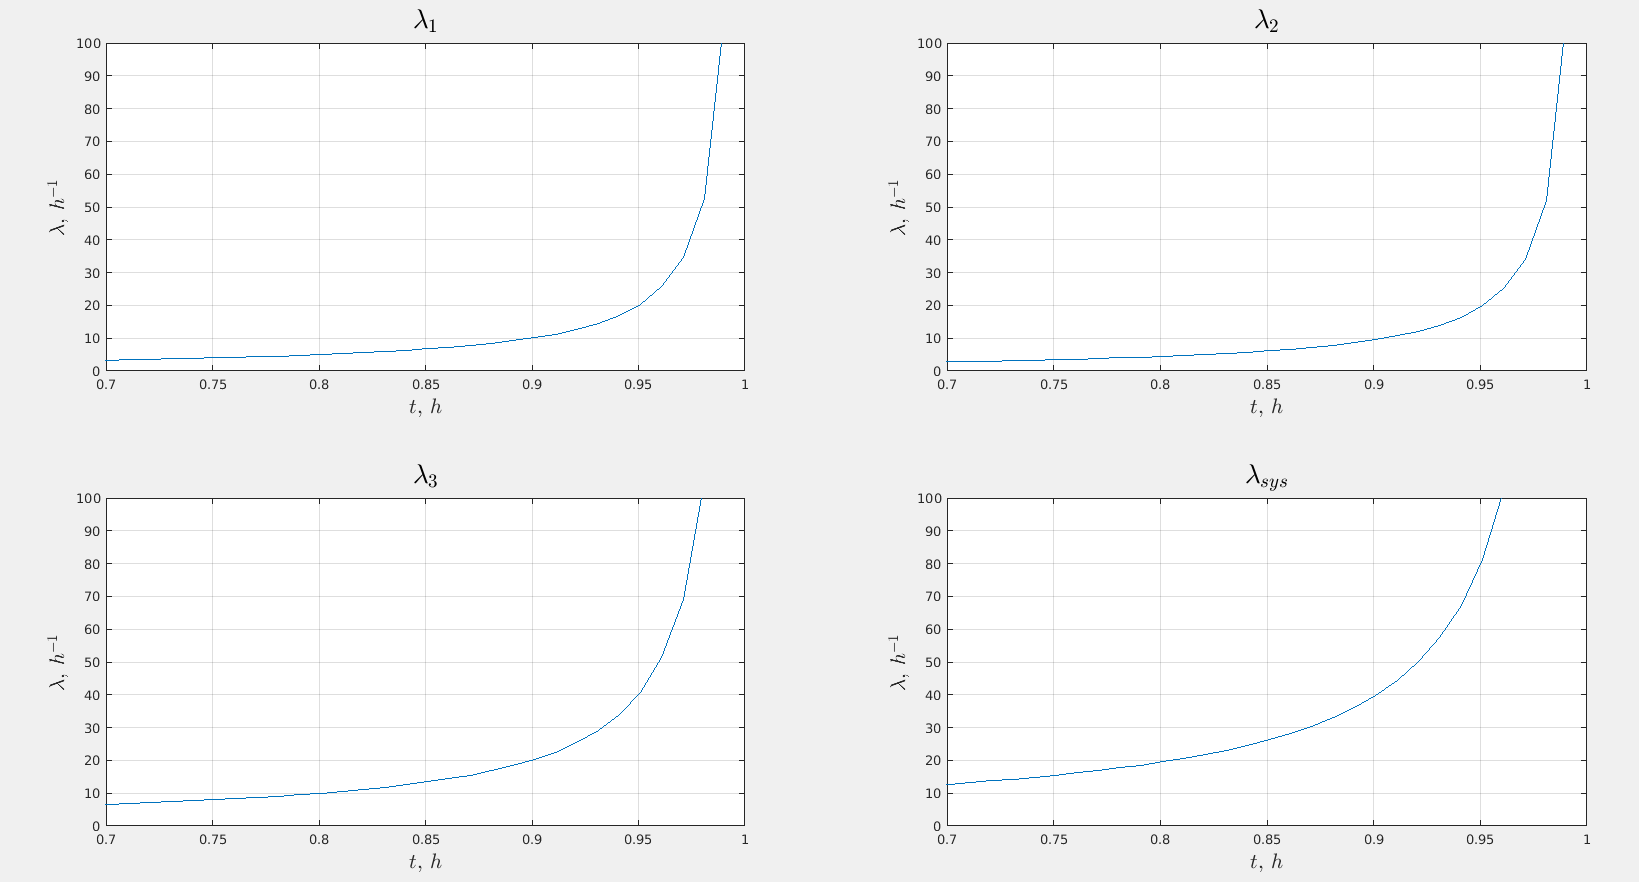
\includegraphics[width=\linewidth]{assets/plots}
  \caption{Интесивность откзов $\lambda_{1}, \lambda_{2}, \lambda_{3}, \lambda_{sys}$}
  \label{img:21-0}
\end{figure}